Este capítulo tem como objetivo apresentar os resultados obtidos pelos procedimentos descritos no
Capítulo~\ref{metodologia}.
Serão avaliados se os objetivos foram atingidos e serão ressaltados problemas encontrados no desenvolvimento.

\section{Primeira Etapa}

A primeira etapa consiste no treinamento de algoritmos de aprendizado de máquina a partir de base de dados anotada
ruidosamente, replicando assim o trabalho de Go \textit{et al.}
Nesta fase foram utilizados o dados disponibilizados no Sentiment140 para treinamento e teste do algoritmo.
Os dados de treinamento são compostos por supervisão distante, totalizando 800 mil exemplos, metade positivos e metade
negativos.
Entretanto, a base de teste dispõe apenas de 360 observações, também divididas igualmente entre as classes.
O baixo número de exemplos pode causar pequenas variações nos resultados obtidos.

Para seleção de hiperparâmetros foram treinados modelos de Naïve Bayes com diferentes fatores de regularização por
suavização de distribuição de laplace.
O modelo selecionado foi o que obteve maior valor médio de acurácia entre 10 partições de validação cruzada.
A Figura~\ref{fig:go_nb} mostra a resposta da acurácia dos diferentes modelos nos grupos de validação, as barras de erro
correspondem a um desvio padrão.
A linha vertical vermelha presente na Figura~\ref{fig:go_nb} indica o melhor parâmetro obtido, aproximadamente 4,1,
resultando em uma acurácia média sobre o conjunto de validação de 78,2\%.
Aplicando-se o modelo de melhor desempenho no conjunto de testes foi obtida acurácia de 83,3\%, este valor se aproxima
ao obtido originalmente: 81,3\%.

\begin{figure}
\begin{center} {
    \begin{center}
    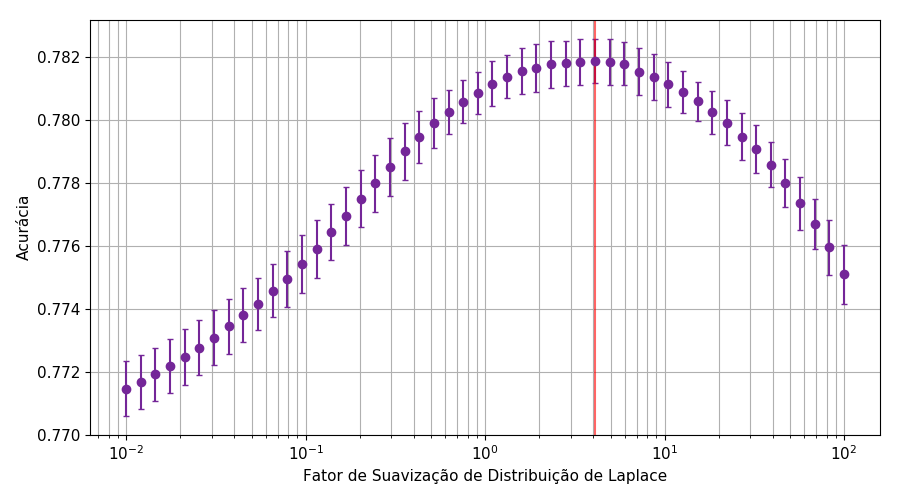
\includegraphics[scale=0.5]{go_nb.png}
    \caption{Seleção de hiperparâmetros de Naïve Bayes - Etapa 1.}
    \label{fig:go_nb}
    \end{center}
}
\end{center}
\end{figure}

A seleção do parâmetros do modelo formado por \textit{Support Vector Machines} foi feita por processo semelhante ao
anterior.
Foram variados o fator de regularização $L_{2}$, selecionando o modelo de maior percentual de acurácia.
A Figura~\ref{fig:go_svm} apresenta os resultados obtidos, no qual o fator de $6 \times 10^{-6}$ resultou na acurácia
média de 80.0\% sobre o conjunto de validação.
O modelo selecionado apresenta 83,0\% de acurácia no conjunto de testes.

\begin{figure}
\begin{center} {
    \begin{center}
    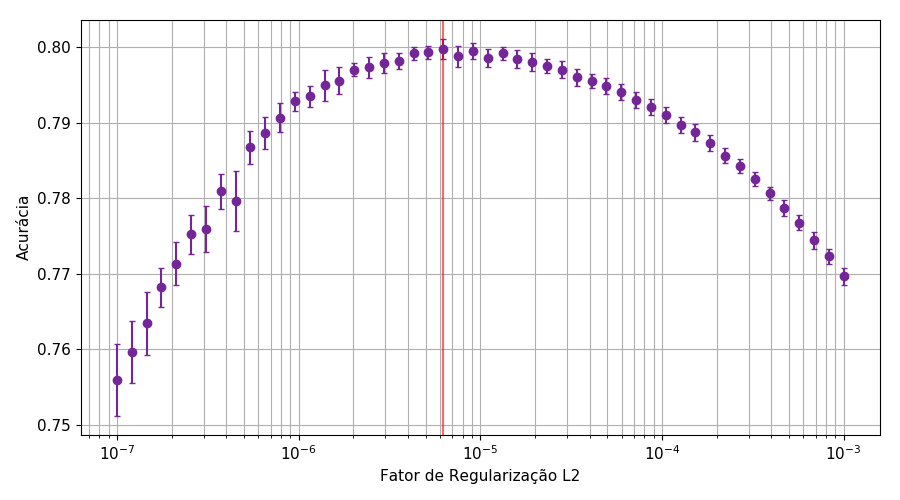
\includegraphics[scale=0.5]{go_svm.png}
    \caption{Seleção de hiperparâmetros de SVM - Etapa 1.}
    \label{fig:go_svm}
    \end{center}
}
\end{center}
\end{figure}

A Tabela~\ref{tab:go_compara} apresenta os resultados obtidos tanto no Sentiment140 quanto pela replicação de
seu método.
Pode se observar que foram atingidos valores próximos a referência, validando assim os pré-processamentos e as
implementações dos algoritmos aplicados.

% Resultados pós calibração
\begin{table}[h]
    \begin{center}
        \begin{tabular}{| l | r | r |}
        \hline
        \textbf{Algoritmo} & \textbf{Original} & \textbf{Replicação} \\ \hline
        Naïve Bayes & 81,3\% & 83,3\% \\ \hline
        SVM &  82,2\% & 83,0\% \\ \hline
        \end{tabular}
        \caption{Comparação de resultados da replicação dos classificadores do Sentiment140.}
        \label{tab:go_compara}
    \end{center}
\end{table}

\section{Segunda Etapa}

A segunda etapa consiste na validação do processo de formação de base de treinamento por supervisão distante.
A aplicação de técnicas de pré-processamento e algoritmos previamente validados neste novo conjunto de dados visa tanto
comparar o processo de elaboração por anotação ruidosa quanto servir como referência para a aplicação de algoritmos de
\textit{Deep Learning}.
Nesta etapa, os modelos serão avaliados tanto pelo seu desempenho na base de teste disponibilizada por Go
\textit{et al.} quanto quando aplicado na base de testes formada pela coletânea de \textit{tweets} oferecida pelas
conferências SemEval, como descrito na Seção~\ref{sec:data}

Assim como na fase anterior, foram treinados modelos por Naïve Bayes e \textit{Support Vector Machines}.
Neste caso, a seleção dos parâmetros de regularização foi feita de maneira a maximizar a área sob a curva ROC.
As Figuras~\ref{fig:nb_selecao} e~\ref{fig:svm_selecao} mostram a resposta dos modelos, respectivamente, Naïve Bayes e
SVM a mudanças nos parâmetros de regularização, as linhas verticais vermelhas apontam os parâmetros que obtiveram maior
média de área sob a curva ROC dentre os grupos de validação quando aplicada validação cruzada com 10 partições.

\begin{figure}
\begin{center} {
    \begin{center}
    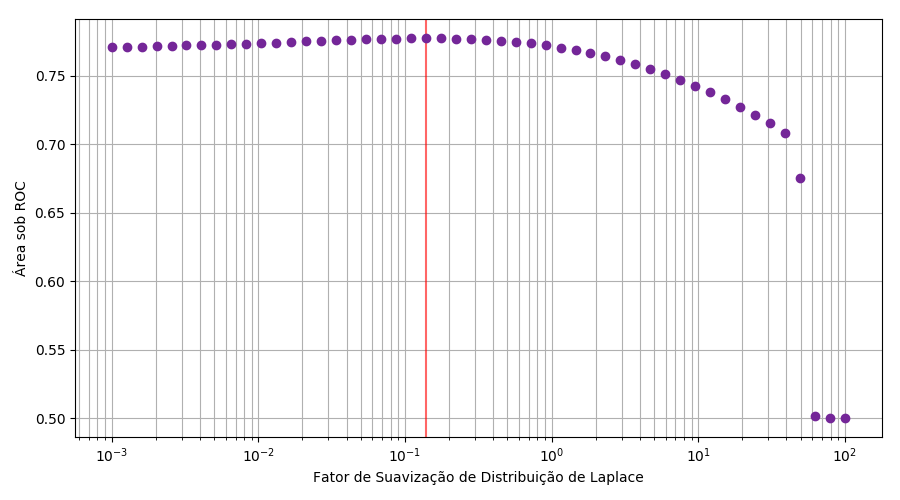
\includegraphics[scale=0.5]{nb_selecao.png}
    \caption{Seleção de hiperparâmetros de Naïve Bayes - Etapa 2.}
    \label{fig:nb_selecao}
    \end{center}
}
\end{center}
\end{figure}

\begin{figure}
\begin{center} {
    \begin{center}
    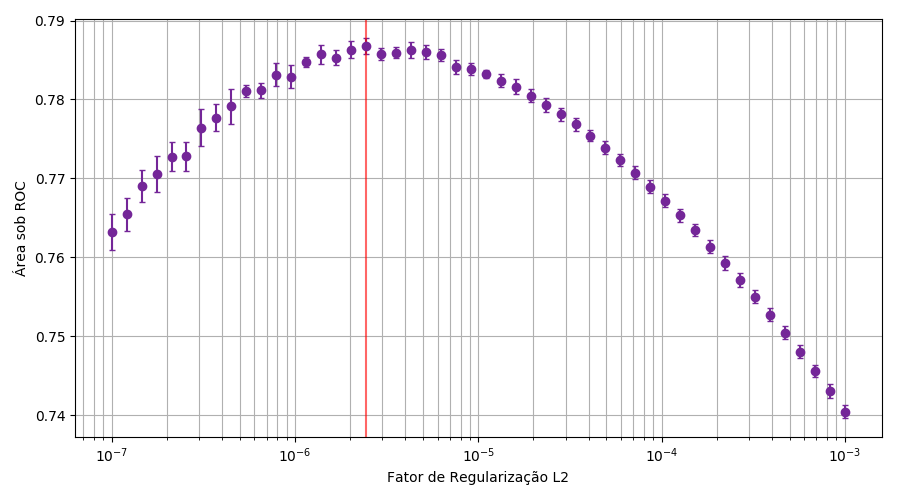
\includegraphics[scale=0.5]{svm_selecao.png}
    \caption{Seleção de hiperparâmetros de SVM - Etapa 2.}
    \label{fig:svm_selecao}
    \end{center}
}
\end{center}
\end{figure}

Uma vez selecionado os melhores hiperparâmetros, a Figura~\ref{fig:linear_roc_go} compara a curva ROC que caracteriza a
performance dos modelos treinandos tanto na primeira quanto na segunda etapa sob os dados de testes disponibilizados
por Go \textit{et al.}
A Figura~\ref{fig:linear_roc_semeval} por sua vez apresenta a curva ROC dos modelos quando aplicados nos dados
manualmente anotados coletados do SemEval.

\begin{figure}
\begin{center} {
    \begin{center}
    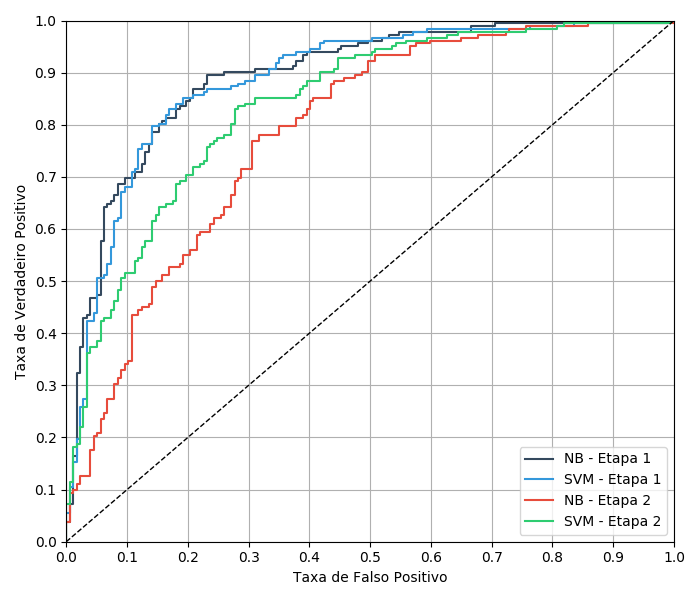
\includegraphics[scale=0.5]{linear_roc_go.png}
    \caption{Curva ROC dos modelos aplicados aos dados de teste do Sentiment140.}
    \label{fig:linear_roc_go}
    \end{center}
}
\end{center}
\end{figure}

\begin{figure}
\begin{center} {
    \begin{center}
    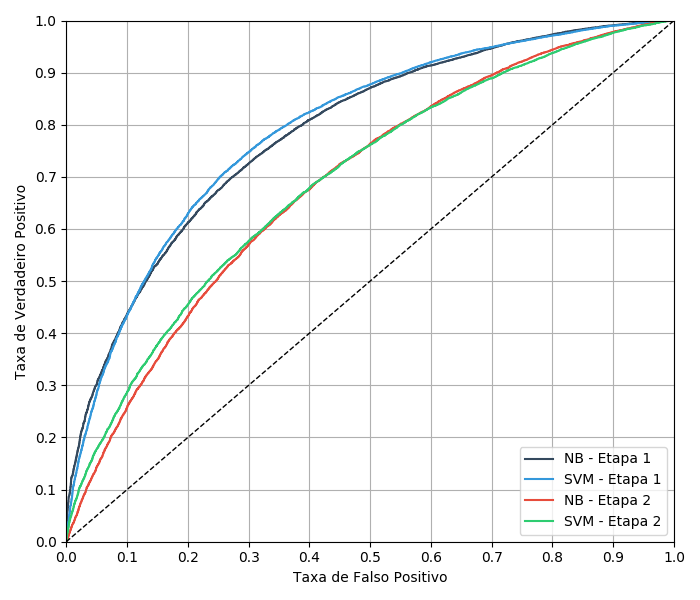
\includegraphics[scale=0.5]{linear_roc_semeval.png}
    \caption{Curva ROC dos modelos aplicados aos dados de teste do SemEval.}
    \label{fig:linear_roc_semeval}
    \end{center}
}
\end{center}
\end{figure}

Observa-se que os modelos treinados pelo conjunto de dados de anotação ruidosa disponibilizados por Go
\textit{et al.} apresentou desempenho consideravelmente melhor nos dois conjuntos de testes.
Desta maneira, se percebe que o processo de anotação dos dados foi mais ruidoso do que o apresentado pelo Sentiment140.

Uma hipótese a ser feita é que evoluções no idioma e na plataforma durante o intervalo entre a criação de ambas as
bases anotadas por supervisão distante tenha dificultado este processo, visto que a desenvolvida por Go \textit{et al.}
foi coletada em 2009, e a base de treinamento coletada por este trabalho conta com \textit{tweets} de 2017.
Constatou-se, por exemplo, que a base desenvolvida neste trabalho apresentou 1,1 milhões de palavras únicas após o
processo de tokenização, enquanto os dados de treinamento do Sentiment140 contam com 330 mil palavras únicas.

Outro fator relevante para definição de ruído no processo de anotação é a escolha dos \textit{emoticons}.
Neste trabalho, além dos \textit{emoticons} utilizados pelo Sentiment140, os \textit{emoticons} mais presentes nos dados
foram selecionados para classificação manual.
A escolha de \textit{emoticons} de maneira a atingir maior correlação com as classes pode ser uma solução para reduzir
a diferença de performance dos modelos entre os resultados de treinamento e os resultados de teste.

Apesar dos resultados obtidos na base de treinamento anotada para este trabalho serem inferiores aos apresentados pelos
classificadores treinados com a base disponibilizada por Go \textit{et al.}, a técnica de supervisão distante por
\textit{emoticons} para anotação ruidosa de mensagens de redes sociais se mantém como boa alternativa ao processo
custoso de anotação manual.

A Tabela~\ref{tab:linear_perf} resume os resultados dos modelos treinados na primeira e na segunda etapas quando
aplicados sob ambos os conjuntos de testes.
O ponto de operação dos modelos foi escolhido de maneira a maximizar o índice SP.
É válido ressaltar que a acurácia é uma métrica inconsistente quando consideras bases de testes com classes
desbalanceadas, como é o caso da base de \textit{tweets} coletados dos SemEval, sendo a área sob a curva ROC, AUC, ou o
índice SP, melhores opções para comparação destes casos.

% AUC -> CalibratedClassifier
% Acurácia, SP -> treshold: ponto de maior SP
\begin{table}[h]
    \begin{center}
        \begin{tabular}{ |l|l|l|r|r|r| }
            \hline
            \textbf{Dados de teste} & \multicolumn{2}{|c|}{\textbf{Modelo}}  & \textbf{Acurácia} & \textbf{AUC} & \textbf{SP} \\ \hline
            \multirow{4}{*}{Sentiment140} & \multirow{2}{*}{Etapa 1} & NB  & 83.3\% & 0.893 & 0.831 \\ \cline{3-6}
                                          &                          & SVM & 83.0\% & 0.887 & 0.830 \\ \cline{2-6}
                                          & \multirow{2}{*}{Etapa 2} & NB  & 73.3\% & 0.785 & 0.732 \\ \cline{3-6}
                                          &                          & SVM & 77,7\% & 0,839 & 0,776 \\ \hline
            \multirow{4}{*}{SemEval}      & \multirow{2}{*}{Etapa 1} & NB  & 70,9\% & 0,786 & 0,713 \\ \cline{3-6}
                                          &                          & SVM & 72,8\% & 0,791 & 0,724 \\ \cline{2-6}
                                          & \multirow{2}{*}{Etapa 2} & NB  & 64,9\% & 0,688 & 0,639 \\ \cline{3-6}
                                          &                          & SVM & 64,2\% & 0,693 & 0,640 \\ \hline
        \end{tabular}
        % FIX
        \caption{Resultados obtidos pelos classificadores.}
        \label{tab:linear_perf}
    \end{center}
\end{table}

\section{Terceira Etapa}

A terceira fase do projeto visa a reproduzir redes neurais convolucionais aplicadas a texto e comparar seu desempenho
a algoritmos de aprendizado de máquina consolidados no processamento de linguagem natural, como presentes na etapa
anterior.
Neste estágio, as redes serão treinadas com dados provindos da base anotada por supervisão distante, mesmos dados
utilizados para treinamento dos algoritmos de Naïve Bayes e \textit{Support Vector Machines} da segunda etapa.
Após feita a seleção dos hiperparâmetros, o modelo será avaliado aos treinados na segunda etapa com base no seu
desempenho obtido na base de testes disponibilizada pelas conferências SemEval.

Foram variados diversos hiperparâmetros, são eles: número de camadas, número de filtros convolucionais por camada,
tamanho dos filtros convolucionais, tamanho do filtro de \textit{pooling}.
Outros hiperparâmetros como: fator de regularização $L_{2}$ e probabilidade de Dropout foram mantidos fixos em
respectivamente $10^{-3}$ e $0,5$.
Os modelos foram treinados até que o valor da função custo estabilizar, não se modificando mais do que um valor
arbitrariamente pequeno, $\epsilon$, entre cada época de treinamento.
O valor escolhido de $\epsilon$ foi $10^{-3}$, o qual foi selecionado após a análise de algumas curvas de treinamento.
Por sua vez, aplicou-se \textit{early stopping}, no qual os pesos da rede selecionados foram os correspondentes a época
de menor valor de função custo aplicada ao conjunto de validação.

A escolha dos hiperparâmetros foi feita de maneira a maximizar a área sob a curva ROC nos dados de validação.
A Tabela~\ref{tab:cnn_selection} lista os resultados obtidos por cada configuração treinada.

% apos treino coletar a auc de todos modelos (nos dados de treinamento mesmo), anotar valores na tabela
\begin{table}[h]
    \begin{center}
        \begin{tabular}{| >{\centering\arraybackslash}m{2.5cm} | >{\centering\arraybackslash}m{2.5cm} | >{\centering\arraybackslash}m{2.5cm} | >{\centering\arraybackslash}m{2.5cm}| c |}
        \hline
        \multicolumn{4}{|c|}{\textbf{Hiperparâmetros}} & \textbf{Resultado} \\ \hline
        \textbf{Número de Camadas} & \textbf{Número Filtros Conv.} & \textbf{Tamanho Filtros Conv.} & \textbf{Tamanho Filtros Pooling} & \textbf{AUC} \\ \hline
        \multirow{12}{*}{1} & \multirow{6}{*}{100} & \multirow{3}{*}{2} & 2 & 0.??? \\ \cline{4-5}
                            &                      &                    & 3 & 0.??? \\ \cline{4-5}
                            &                      &                    & 5 & 0.??? \\ \cline{3-5}

                            &                      & \multirow{3}{*}{3} & 2 & 0.??? \\ \cline{4-5}
                            &                      &                    & 3 & 0.??? \\ \cline{4-5}
                            &                      &                    & 5 & 0.??? \\ \cline{2-5}

                            & \multirow{6}{*}{200} & \multirow{3}{*}{2} & 2 & 0.??? \\ \cline{4-5}
                            &                      &                    & 3 & 0.??? \\ \cline{4-5}
                            &                      &                    & 5 & 0.??? \\ \cline{3-5}

                            &                      & \multirow{3}{*}{3} & 2 & 0.??? \\ \cline{4-5}
                            &                      &                    & 3 & 0.??? \\ \cline{4-5}
                            &                      &                    & 5 & 0.??? \\ \cline{1-5}

        \multirow{12}{*}{2} & \multirow{6}{*}{100} & \multirow{3}{*}{2} & 2 & 0.??? \\ \cline{4-5}
                            &                      &                    & 3 & 0.??? \\ \cline{4-5}
                            &                      &                    & 5 & 0.??? \\ \cline{3-5}

                            &                      & \multirow{3}{*}{3} & 2 & 0.??? \\ \cline{4-5}
                            &                      &                    & 3 & 0.??? \\ \cline{4-5}
                            &                      &                    & 5 & 0.??? \\ \cline{2-5}

                            & \multirow{6}{*}{200} & \multirow{3}{*}{2} & 2 & 0.??? \\ \cline{4-5}
                            &                      &                    & 3 & 0.??? \\ \cline{4-5}
                            &                      &                    & 5 & 0.??? \\ \cline{3-5}

                            &                      & \multirow{3}{*}{3} & 2 & 0.??? \\ \cline{4-5}
                            &                      &                    & 3 & 0.??? \\ \cline{4-5}
                            &                      &                    & 5 & 0.??? \\ \cline{1-5}

        \end{tabular}
    \caption{Seleção de hiperparâmetros de CNN.}
    \label{tab:cnn_selection}
    \end{center}
\end{table}

De acordo com a tabela, podemos observar que o conjunto de parâmetros com melhor desempenho no conjunto de validação
foram: X camadas compostas por Y filtros convolucionais de tamanho Z seguidas de \textit{pooling} com filtro de tamanho
W.
A Figura XYZ mostra a curva de treinamento deste modelo.

% figura de treinamento com loss x val_loss, com legenda de cores e ressaltando a epoca selecionada

Uma vez selecionados os hiperparâmetros da rede neural convolucional, a Figura XYZ apresenta a curva ROC comparativa
entre a rede e os modelos treinandos na segunda etapa quando aplicados a base de testes formada por \textit{tweets}
fornecido pelas conferências SemEval.
A Tabela XYZ resume os resultados destes classificadores, novamente considerando que o limiar de decisão foi selecionado
de maneira a maximizar o índice SP.

FIGURA CURVA ROC - NB x SVM x CNN

TABELAS RESULTADOS (AUC, SP)  NB x SVM x CNN

Pode se observar que a utilização de redes neurais convolucionais em conjunto com representações obtidas por
\textit{embeddings} propiciou resultados melhores do que os obtidos com modelos tradicionais, como Naïve Bayes e
\textit{support vector machines} sobre representações \textit{one-hot} dos textos.
Ressalta-se que a representação Word2Vec utilizada foi desenvolvida a partir de notícias.
O treinamento de modelos próprios para o meio no qual serão utilizados, neste caso, \textit{tweets}, pode melhorar o
desempenho do classificador a ser utilizado.
